% Drawing 70/04-5 -- folder 70, batch 04, archive page 74 (PDF page 75).
% Transcription: Seconde figure : l'icosaèdre projeté dans le triangle $\bar s_1, \bar s_0, \bar s_2$, avec au centre $s_0, s_1, s_2, s_3, s'_3, s''_3$, $\bar s_3$, $\bar s'_3$, $\bar s''_3$ ; esquisse au crayon dessous.
% Kind: icosahedron projected in a triangle. Method 3 (encoded, rendered from the data). Status: ok.
% Notes: The icosahedron in Schlegel projection from the face s-bar_1 s-bar_0 s-bar_2 (the outer triangle): inside, the large triangle s-bar_3 (top), s-bar''_3 (left), s-bar'_3 (right); s'_3, s''_3, s_3 at the midpoints of its sides (they lie on its sides on the page); the central face s_0 s_1 s_2 with s_2 on the segment s'_3 s''_3. Every edge is drawn between the 12 vertices, so the 30 edges meet exactly at them: each outer vertex joined to its 3 neighbours on the middle ring, s_2 to s'_3, s''_3, s-bar_3, s_0 to s'_3, s_3, s-bar''_3, s_1 to s''_3, s_3, s-bar'_3. The combinatorics is checked as a polyhedron (12 vertices, 30 edges, 20 faces). On the page the edges s_0 s_3 and s_1 s_3 are slightly bowed and the line s-bar''_3 s_0 s_1 s-bar'_3 is drawn in one stroke; here they are straight. Left out: the faint pencil construction lines under the ink, and the long pencil curve under the figure (it separates the figure from the formulas below). Labels: s-bar_1 is written without a visible bar, s-bar''_3 too; they are given the transcription's bars. Nothing is struck in this figure. Redrawn 2026-11-09 (issue 128) after Michel's check: vertices placed once and every edge drawn between them, so concurrent lines meet exactly; labels at \small. Revised 2026-11-09 after Michel's check (#131): Michel accepted the redraw as it stands (bars as in the transcription).
% Coordinates: 1 unit = 1 mm = 1/100 of the crop width (bbox in page fractions: [0.07, 0.25, 0.4, 0.405]).
% Redrawn by Claude (claude-opus-5-5), issue #73, 2026-11-09; not checked by a human; not compiled (no TeX in the session).
% Rights: reproduces part of the work -- behind RENDER_TRANSCRIPTS, never published by itself.
\documentclass[tikz,border=3pt]{standalone}
\usepackage{amsmath,amssymb}
\usetikzlibrary{patterns,arrows.meta}
\tikzset{pencil/.style={black!45}, struck/.style={black!35}, mark/.style={circle,draw,inner sep=1.3pt}, pt/.style={circle,fill,inner sep=0.9pt}, opt/.style={circle,draw,fill=white,inner sep=1.1pt}}
\begin{document}
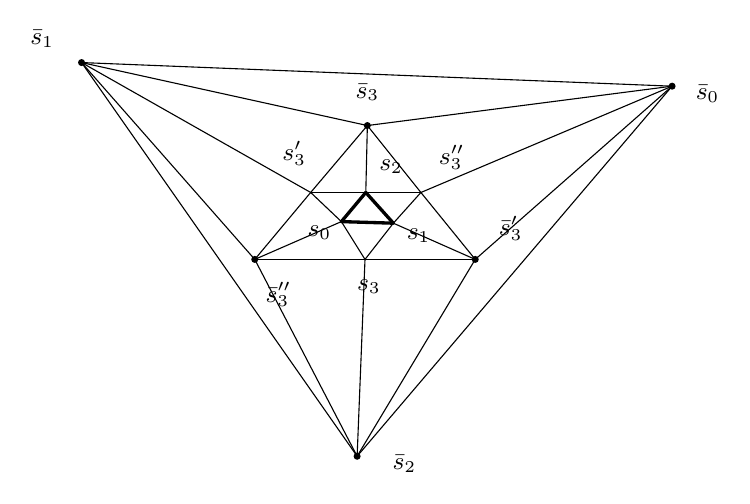
\begin{tikzpicture}[x=1mm,y=1mm,line cap=round,line join=round,font=\scriptsize]
\draw (19,-6) -- (94,-9);
\draw (94,-9) -- (54,-56);
\draw (54,-56) -- (19,-6);
\draw[very thick] (52,-26.2) -- (58.6,-26.4);
\draw[very thick] (58.6,-26.4) -- (55.1,-22.5);
\draw[very thick] (55.1,-22.5) -- (52,-26.2);
\draw (55.1,-22.5) -- (48.1,-22.5);
\draw (55.1,-22.5) -- (62.1,-22.5);
\draw (55.1,-22.5) -- (55.3,-14);
\draw (52,-26.2) -- (48.1,-22.5);
\draw (52,-26.2) -- (55,-31);
\draw (52,-26.2) -- (41,-31);
\draw (58.6,-26.4) -- (62.1,-22.5);
\draw (58.6,-26.4) -- (55,-31);
\draw (58.6,-26.4) -- (69,-31);
\draw (55.3,-14) -- (62.1,-22.5);
\draw (62.1,-22.5) -- (69,-31);
\draw (69,-31) -- (55,-31);
\draw (55,-31) -- (41,-31);
\draw (41,-31) -- (48.1,-22.5);
\draw (48.1,-22.5) -- (55.3,-14);
\draw (55.3,-14) -- (19,-6);
\draw (55.3,-14) -- (94,-9);
\draw (62.1,-22.5) -- (94,-9);
\draw (69,-31) -- (94,-9);
\draw (69,-31) -- (54,-56);
\draw (55,-31) -- (54,-56);
\draw (41,-31) -- (54,-56);
\draw (41,-31) -- (19,-6);
\draw (48.1,-22.5) -- (19,-6);
\node[pt] at (19,-6) {};
\node[pt] at (94,-9) {};
\node[pt] at (54,-56) {};
\node[pt] at (55.3,-14) {};
\node[pt] at (69,-31) {};
\node[pt] at (41,-31) {};
\node[inner sep=1pt] at (14,-3) {\small $\bar s_1$};
\node[inner sep=1pt] at (98.5,-10) {\small $\bar s_0$};
\node[inner sep=1pt] at (60,-57) {\small $\bar s_2$};
\node[inner sep=1pt] at (55.3,-9.8) {\small $\bar s_3$};
\node[inner sep=1pt] at (73.5,-27) {\small $\bar s'_3$};
\node[inner sep=1pt] at (44,-35.5) {\small $\bar s''_3$};
\node[inner sep=1pt] at (46,-17.5) {\small $s'_3$};
\node[inner sep=1pt] at (66,-18) {\small $s''_3$};
\node[inner sep=1pt] at (55.5,-34.5) {\small $s_3$};
\node[inner sep=1pt] at (49.2,-27.6) {\small $s_0$};
\node[inner sep=1pt] at (61.8,-28) {\small $s_1$};
\node[inner sep=1pt] at (58.3,-19.2) {\small $s_2$};
\end{tikzpicture}
\end{document}
